\section{Operating System Selection Process}

We wanted to ensure that we had the same operating system configuration across all configurations, and to that end we started testing out different distributions to figure out which one would be the best for our purposes.\\

We wanted to make sure we made an informed decision when it came to our platform, and as such we did a number of tests on other operating systems in order to ensure that we made the correct choice.\\

Initially, we decided to eliminate and narrow down our choices, as the amount of Linux distributions available would make this process in itself take up most of our time. So in order to limit the time spent on this task, we decided to select the most common and mainstream Linux distributions, which effectively narrowed it down to Fedora, Ubuntu, and OpenSUSE in addition to the vendor-supplied Raspberry Pi OS. \\

Then we decided to look at what our architecture should look like with the software running on the different hardware configurations and how we would ensure a uniform configuration across all our running systems. A decision was made to run everything within containers, this would ensure that libraries and versions of software running would be identical across all systems. As a container system, we opted to go for Docker, as this is the most used and the most common configuration out there, and it is well supported on all the platforms we evaluated, and our team already had some knowledge of how to best utilize docker to our advantage.  \\

For the software for communicating between the different parts of our system, we opted to use Robot Operating System version 2 (ROS2). This is a ready-to-run turnkey solution for setting up robots or drones, it makes it easy to communicate between different parts of our system, and it is network aware as well as having a communications system between ROS2 instances running within a Docker environment.\\


After deciding which configurations to explore, we started by systematically installing the different distributions on physical hardware, and examining what functionality worked and what did not. From figure \ref{fig:osarch} you can see the different results and what worked and what did not. \\ 

\begin{figure}[h]
    \centering
    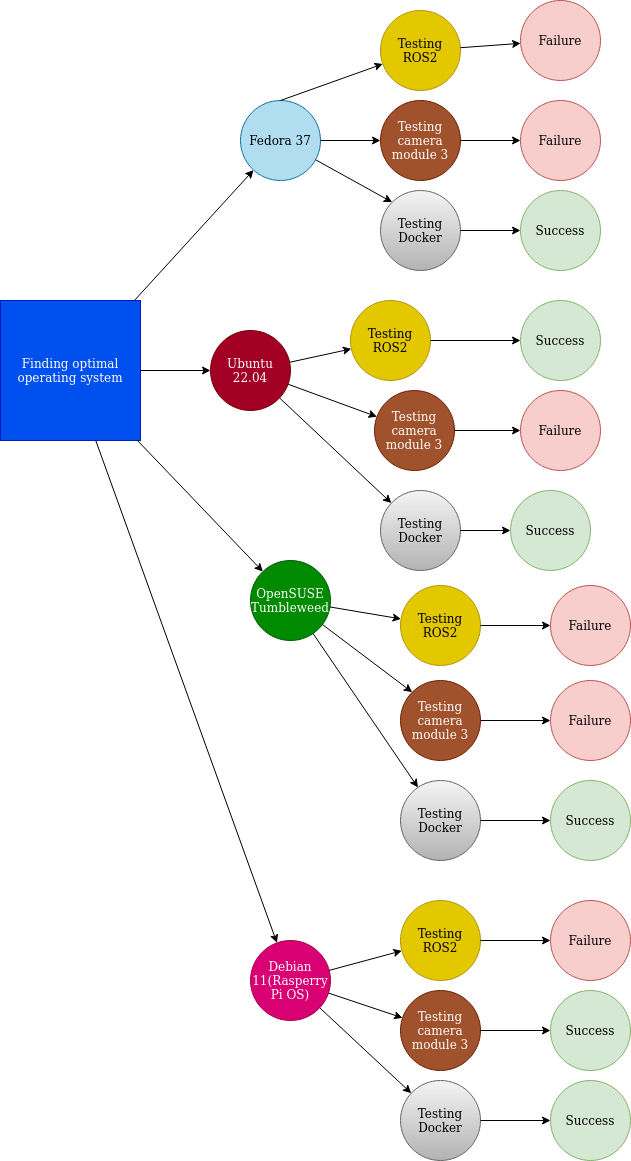
\includegraphics[scale=0.5]{fig/decision_os.png}
    \caption{Decision Process OS}
    \label{fig:osarch}
\end{figure}


As indicated in the figure, there were no systems that met all the requirements we had for our software platform, this caused a need to do further research in order to be able to decide which platform we would use going forward. \\

We further narrowed down our choices to Ubuntu or Debian, as these platforms only had one missing dependency, however, we needed to determine which path would yield the best results in contrast to the work needed to fix each system.\\

\begin{figure}[h]
    \centering
    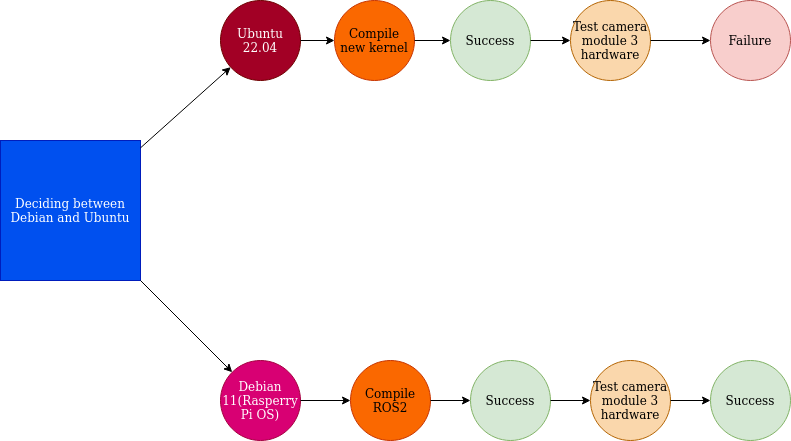
\includegraphics[scale=0.5]{fig/select_dist.png}
    \caption{Decision Process Distribution}
    \label{fig:distselect}
\end{figure}

Debian had the disadvantage of having problems getting ROS2 to work, which has a fairly complicated and extensive build-system, where the documentation can be outdated due to how fast the ROS2 project moves at this point in time. On the other hand, the challenge posed by the Ubuntu system was the absence of driver software for the camera module version 3. \\

As we had limited experience with the ROS2 build system, and documentation on how to manually build and install the software was sparse, we decided to attempt to install the existing driver from Debian in a Ubuntu environment, in order to run ROS2 with camera version 3. \\

We started by cloning the git repository from the Raspberry Pi foundation, where we knew there was a working driver, as our initial tests with Debian showed this to be the case. After cloning the repository we cross-compiled the kernel configuration along with the necessary libraries for installation on our Ubuntu system. \\

After finishing the installation and booting our new kernel, the hardware was detected, but there was no video output. At this point, it was our opinion that we could still get the hardware to function under Ubuntu, as that would be our best course of action at this moment in time. \\

We continued to perform different tests with different configurations, as well as compiling different versions of the Linux kernel, including a vanilla upstream version. When none of these approaches yielded the results we needed, we were forced to re-evaluate our attack vector for this problem.\\

We revisited the drawing board and had a look at running ROS2 on our Debian system, which would provide us access to the camera module 3 driver, and would simplify the deployment of our software. \\

After deciding to attempt a ROS2 compile for Debian, we dove into the documentation for compiling the software on our system, however, this proved less than straightforward and we had numerous challenges attempting to get the software to compile. As an intermediary solution, we found someone who had compiled a Debian package for us on github, but this was from an older build and we could not verify it for our uses, leaving us with the necessary steps to continue to deploy ROS2 while we had an insecure installation with ROS2 for other group members so we could work in parallel and speed up development.\\

After a long period of non-stop work, we were able to compile ROS2 under a Debian system, allowing us access to the camera module 3 and ROS2 on the same computer. After this step was done, we needed to deploy this to a Docker image, allowing us to control the environment and secure a cohesive and uniform platform for our ROS2 source code.\\



However, an unfortunate side-effect of compiling software is that it grows rather large, and after building our Docker system, it had increased in size to 14GB, which was unwieldy for deployment and it posed a challenge to run on the Raspberry Pi Zero. This was sadly nothing we were able to rectify in time before delivering our project, and while it does work in the Raspberry Pi Zero, deployment is slow and prone to create problems if the Zero runs out of memory while pulling the Docker image.\\